\documentclass[10pt]{article}

% =============================================================================
% DATOS GENERALES DEL TRABAJO
% =============================================================================
\newcommand{\materia}{Instrumentación Biomédica I}
\newcommand{\institucion}{Instituto Tecnológico de Buenos Aires}
\newcommand{\numeroTP}{2}
\newcommand{\nombreTP}{Sensor de Temperatura}
\newcommand{\anioTP}{2026}

% =============================================================================
% FORMATO EXIGIDO POR LA CÁTEDRA
% =============================================================================
\textheight=21cm
\textwidth=15cm
\topmargin=-0.5cm
\oddsidemargin=1cm
\evensidemargin=1cm
\parindent=0mm

% =============================================================================
% PAQUETES
% =============================================================================

% Codificación e idioma
\usepackage[utf8]{inputenc}
\usepackage[T1]{fontenc}
\usepackage[spanish,es-tabla]{babel}

% Matemática y unidades
\usepackage{amsmath,amssymb}
\usepackage{siunitx}
\sisetup{output-decimal-marker={,}}

% Figuras y tablas
\usepackage{graphicx}
\graphicspath{{imagenes/}}
\DeclareGraphicsExtensions{.pdf,.png,.jpg,.jpeg}
\usepackage{float}
\usepackage{subcaption}
\usepackage{booktabs}
\usepackage{array}
\usepackage{adjustbox}

% Formato de página
\usepackage{fancyhdr}
\usepackage{multicol}
\usepackage{xcolor}

% Enlaces y referencias
\usepackage[hidelinks]{hyperref}

% =============================================================================
% CONFIGURACIÓN GENERAL
% =============================================================================
\newcommand{\HRule}{\rule{\linewidth}{0.5mm}}

\pagestyle{fancy}
\fancyhf{}
\setlength{\headheight}{28pt}
\fancyhead[L]{Instrumentación Biomédica I - ITBA}
\fancyhead[R]{TP 2}
\fancyfoot[C]{\thepage}

\begin{document}

% =============================================================================
% CARÁTULA
% =============================================================================
\begin{center}

\textsc{\LARGE \materia}\\[0.2cm]
\textsc{\Large \institucion}\\[0.2cm]

\HRule \\[0.2cm]
{\huge\bfseries TP \numeroTP{} - \nombreTP \\[0.2cm]}
\HRule \\[1cm]

\begin{multicols}{2}

% Profesores
\begin{flushleft}
    \large
    \textbf{Profesores:}\\
    Hernán \textsc{Soares}\\
    Sofía \textsc{Cerretini}
\end{flushleft}

\columnbreak

% Integrantes
\begin{flushleft}
    \large
    \textbf{Alumnos/as:}\\
    Joaquín \textsc{Basualdo} -- 65658\\
    Bautista \textsc{Estrada} -- 65583\\
    Facundo \textsc{Garaguso Fernandez} -- 65436\\
    Augusto \textsc{Frate} -- 65013
\end{flushleft}

\end{multicols}

\vspace{0.5cm}

\renewcommand{\arraystretch}{1.6}

\begin{adjustbox}{max width=\textwidth}
\begin{tabular}{|p{6cm}|p{7cm}|}
\hline
\textbf{Criterio} & \textbf{Calificación} \\ \hline
Presentación & \\ \hline
Desarrollo & \\ \hline
Conclusiones & \\ \hline
Nota Final & \\ \hline\hline
Firma y Fecha & \\ \hline
\end{tabular}
\end{adjustbox}

\end{center}

\thispagestyle{fancy}

% =============================================================================
% ÍNDICE
% =============================================================================
\newpage
\tableofcontents
\thispagestyle{fancy}

\newpage

% =============================================================================
% INFORME
% El cuerpo principal debe ocupar entre 2 y 4 carillas, sin contar carátula,
% índice, anexo ni bibliografía.
% =============================================================================

\section{Objetivo}

El objetivo del trabajo es comprender el comportamiento de un sensor NTC de
\SI{10}{\kilo\ohm} y analizar su utilización para la medición de temperatura.
Para ello se estudia la relación entre resistencia y temperatura, se simula el
circuito de medición, se realiza una medicion experimental mediante
mediciones de resistencia y temperatura con multímetro y termocupla, y se implementa la adquisición mediante Arduino utilizando
la ecuación de Steinhart--Hart.

\section{Desarrollo}

\subsection{Caracterización experimental del termistor}

Para caracterizar experimentalmente el termistor se midieron tres condiciones de
temperatura: ambiente, agua con hielo y agua caliente. En cada caso, la temperatura
se determinó mediante la termocupla conectada al multímetro, colocando simultáneamente
el termistor en el mismo medio. Una vez estabilizada la medición de temperatura, se
midió la resistencia del termistor con el multímetro.

\vspace{0.3cm}

De esta forma se obtuvieron tres pares resistencia--temperatura, correspondientes a
\SI{20}{\celsius} y \SI{8.12}{\kilo\ohm} para temperatura ambiente,
\SI{1}{\celsius} y \SI{17}{\kilo\ohm} para agua con hielo, y
\SI{78}{\celsius} y \SI{6.2}{\kilo\ohm} para agua caliente. Los resultados se
presentan en la Tabla~\ref{tab:mediciones_ntc} del Anexo.

\subsection{Medición mediante Arduino con parámetros nominales}

Luego se implementó la medición digital conectando el termistor en serie con una
resistencia de \SI{10}{\kilo\ohm} y llevando la tensión del punto medio del divisor
a una entrada analógica del Arduino, según el circuito mostrado en la
Figura~\ref{fig:circuito_arduino}. Mediante su conversor analógico--digital (ADC),
la tensión medida fue procesada por software para obtener la resistencia del
termistor y estimar su temperatura.
\vspace{0.3cm}

Inicialmente se utilizaron los parámetros nominales indicados en la hoja de datos
del sensor. Se repitieron las tres condiciones anteriores: temperatura ambiente,
agua con hielo y agua caliente. Los resultados obtenidos se presentan en la
Tabla~\ref{tab:mediciones_arduino_nominal} del Anexo.

% Describir el procedimiento, desarrollo teórico y análisis experimental.
% Todo resultado debe estar acompañado por su justificación teórica.
%
% Ejemplo para insertar una figura desde la carpeta imagenes/:
%
% \begin{figure}[H]
%     \centering
%     \includegraphics[width=0.75\textwidth]{nombre_imagen.png}
%     \caption{Descripción de la figura.}
%     \label{fig:ejemplo}
% \end{figure}
%
% Para referenciarla en el texto:
% Figura~\ref{fig:ejemplo}.

\subsection{Medición mediante Arduino con parámetros propios}
Utilizando los valores experimentales obtenidos con el termistor, se utilizó la página web de Rusefi para la resolución de la ecuación de Steinhart-Hart, con los valores de temperatura y resistencia anotados.
A pesar de que, idealmente, el valor más bajo medido debería ser de 0 grados Celsius y el valor más alto de aproximadamente 50 grados Celsius, se emplearon los valores medidos para resolver la cuenta.
\vspace{0.3cm}

Los parámetros obtenidos y los nominales y los resultados para temperatura y resistencia obtenidos con el módulo Arduino se pueden ver las Tablas \ref{tab:constantes_steinhart_hart} y \ref{tab:mediciones_arduino_experimental} del anexo, respectivamente.
\vspace{0.3cm}

Resulta evidente al observar las constantes teóricas y las obtenidas y compararlas que A y C son positivas en un caso, y negativas en el otro, dando indicios de un posible problema en la obtención de estos. Sin embargo, sólo se puede asegurar que hubo un error al realizar nuevamente las mediciones de temperatura y resistencia.
Finalmente, se observa una diferencia considerable con las mediciones previas de temperatura, pues en este caso se obtuvieron valores imposibles. Por otro lado, las resistencias resultan coherentes. Esto es porque los valores no son calculados mediante la ecuación de Steinhart-Hart, haciendo que no se vean afectados.
Esto se puede deber a errores en las temperaturas usadas (es decir, no haber llegado a las temperaturas máxima y mínima óptimas para la obtención de las constantes) o, más probablemente, a errores de medición.

\section{Conclusiones}

La caracterización experimental confirmó el comportamiento físico propio del termistor NTC, evidenciando una relación resistencia--temperatura decreciente y marcadamente no lineal, coherente con el modelo exponencial de la familia ensayada ($R_{25} = 10\text{ k}\Omega$). Asimismo, se validó la factibilidad del arreglo de divisor resistivo y la adquisición mediante el conversor analógico--digital (ADC) del microcontrolador como método simple y de bajo costo para la digitalización de la variable.

\vspace{0.3cm}

Al implementar la lectura con los parámetros nominales del fabricante, se observó un desajuste sistemático que creció con la distancia al punto de calibración ($25^\circ\text{C}$), alcanzando un error de hasta $\approx 7^\circ\text{C}$ en la condición de agua caliente. Estimaciones de orden de magnitud permiten descartar la resolución del ADC y el autocalentamiento del sensor como causas dominantes de esta discrepancia (ambos efectos resultan órdenes de magnitud menores). Por ende, el error se atribuye al desvío intrínseco de las constantes nominales de catálogo respecto de la curva real del componente.

\vspace{0.3cm}

En el ámbito de la instrumentación biomédica, errores de varios grados Celsius son inaceptables para la monitorización de temperatura corporal (donde se exige exactitud clínica). Teóricamente, esto impone la necesidad de calibrar individualmente cada unidad mediante el ajuste empírico de los tres coeficientes de Steinhart-Hart ($A$, $B$ y $C$) a partir de pares $R$--$T$ relevados antes de su puesta en servicio.

\vspace{0.3cm}

No obstante, la determinación de dichos parámetros empíricos derivó en valores anómalos, con los signos de las constantes $A$ y $C$ invertidos respecto de los teóricos. Este comportamiento se debió a un error experimental en la medición del punto caliente registrada en la Tabla~\ref{tab:mediciones_ntc}, donde se anotó una resistencia de \SI{6.2}{\kilo\ohm} para \SI{78}{\celsius}. Para este sensor NTC, una resistencia de \SI{6.2}{\kilo\ohm} corresponde en realidad a unos \SI{38}{\celsius}, mientras que a \SI{78}{\celsius} el valor físico real debió situarse cercano a \SI{1.7}{\kilo\ohm} (como el propio Arduino registró luego en la Tabla~\ref{tab:mediciones_arduino_nominal}). No se conoce donde se produjo el error durante las mediciones. Por su parte, al forzar al sistema matricial de Steinhart-Hart a ajustar puntos contradictorios con la física del semiconductor, el modelo matemático distorsionó la curvatura polinómica, invirtiendo los signos de las constantes y provocando que las lecturas en Arduino divergieran por completo.

\vspace{0.3cm}

La distorsión del modelo resultó ser total, tal como se ilustra en la Figura~\ref{fig:divergencia_temperaturas}. La discrepancia fue de tal magnitud que resultó sumamente complejo definir una escala gráfica que permitiera comparar con claridad las mediciones: mientras las temperaturas reales y las obtenidas con parámetros nominales oscilaban en el rango biológico y experimental acotado de 0 a \SI{80}{\celsius}, las estimaciones del modelo empírico distorsionado se dispersaron violentamente entre \SI{-901.4}{\celsius} y \SI{146.6}{\celsius}. Esto evidencia de forma gráfica el colapso numérico del algoritmo ante datos de calibración térmicamente incongruentes.
\vspace{0.3cm}

En conclusión, el trabajo práctico demostró que la exactitud final del sistema no está limitada por el conversor analógico--digital ni por la topología del Circuito, sino por la extrema sensibilidad del modelo de Steinhart-Hart frente a la precisión y rigurosidad metodológica con la que se efectúa la calibración individual del transductor.
% cuando corresponda, relacionarlos con aplicaciones en bioingeniería.

% =============================================================================
% BIBLIOGRAFÍA
% No se contabiliza dentro de las 2--4 carillas del cuerpo principal.
% Descomentar y completar cuando se incorporen fuentes externas.
% =============================================================================
%



% =============================================================================
% ANEXO
% No se contabiliza dentro de las 2--4 carillas del cuerpo principal.
% =============================================================================
%
\newpage
\appendix
\section{Anexo}

\subsection{Mediciones de temperatura y resistencia}

\begin{figure}[H]
    \centering
    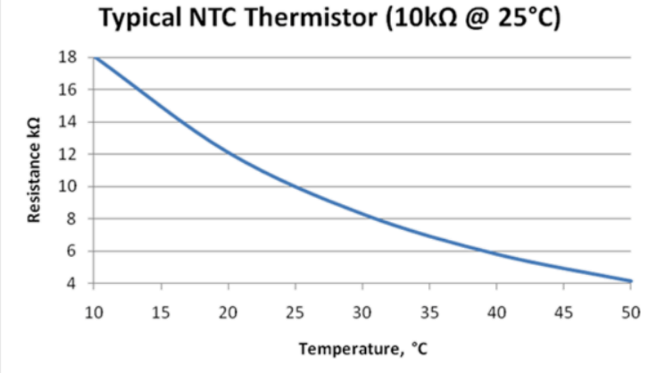
\includegraphics[width=0.92\textwidth]{curva_thermistor.png}
    \caption{Curva característica típica provista por la hoja de datos del fabricante para el termistor NTC ($10\text{ k}\Omega\text{ a }25^\circ\text{C}$).}
    \label{fig:curva_datasheet}
\end{figure}

\begin{table}[H]
    \centering
    \caption{Mediciones experimentales de temperatura y resistencia del termistor.}
    \begin{tabular}{|l|c|c|}
        \hline
         & \textbf{Temperatura} & \textbf{Resistencia} \\ \hline
        Ambiente & \SI{20}{\celsius} & \SI{8.12}{\kilo\ohm} \\ \hline
        Frio & \SI{1}{\celsius} & \SI{17}{\kilo\ohm} \\ \hline
        Caliente & \SI{78}{\celsius} & \SI{6.2}{\kilo\ohm} \\ \hline
    \end{tabular}
    \label{tab:mediciones_ntc}
\end{table}

\subsection{Resultados de la medición con parámetros nominales}

\begin{figure}[H]
    \centering
    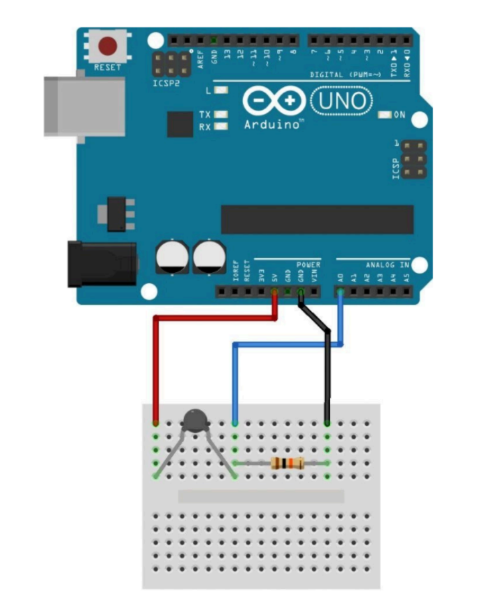
\includegraphics[width=0.88\textwidth]{CircuitoArduino.png}
    \caption{Circuito utilizado para la adquisición de la señal del termistor mediante Arduino.}
    \label{fig:circuito_arduino}
\end{figure}

\begin{table}[H]
    \centering
    \caption{Mediciones obtenidas mediante Arduino utilizando los parámetros nominales del sensor.}
    \begin{tabular}{|l|c|c|}
        \hline
         & \textbf{Temperatura} & \textbf{Resistencia} \\ \hline
        Ambiente & \SI{21.6}{\celsius} & \SI{12164}{\ohm} \\ \hline
        Frio & \SI{3.2}{\celsius} & \SI{29203}{\ohm} \\ \hline
        Caliente & \SI{71}{\celsius} & \SI{1701}{\ohm} \\ \hline
    \end{tabular}
    \label{tab:mediciones_arduino_nominal}
\end{table}

\subsection{Comparación entre parámetros nominales y experimentales del termistor}

\begin{table}[H]
    \centering
    \caption{Comparación entre los valores nominales y experimentales de las constantes de la ecuación de Steinhart-Hart.}
    \begin{tabular}{|c|c|c|}
        \hline
        \textbf{Constante} & \textbf{Valor nominal} & \textbf{Valor experimental} \\ \hline
        $A$ & $1.129148\times10^{-3}$ & $-1.043532\times10^{-1}$ \\ \hline
        $B$ & $2.34125\times10^{-4}$ & $1.714248\times10^{-2}$ \\ \hline
        $C$ & $8.76741\times10^{-8}$ & $-6.381518\times10^{-5}$ \\ \hline
    \end{tabular}
    \label{tab:constantes_steinhart_hart}
\end{table}

\begin{figure}[H]
    \centering
    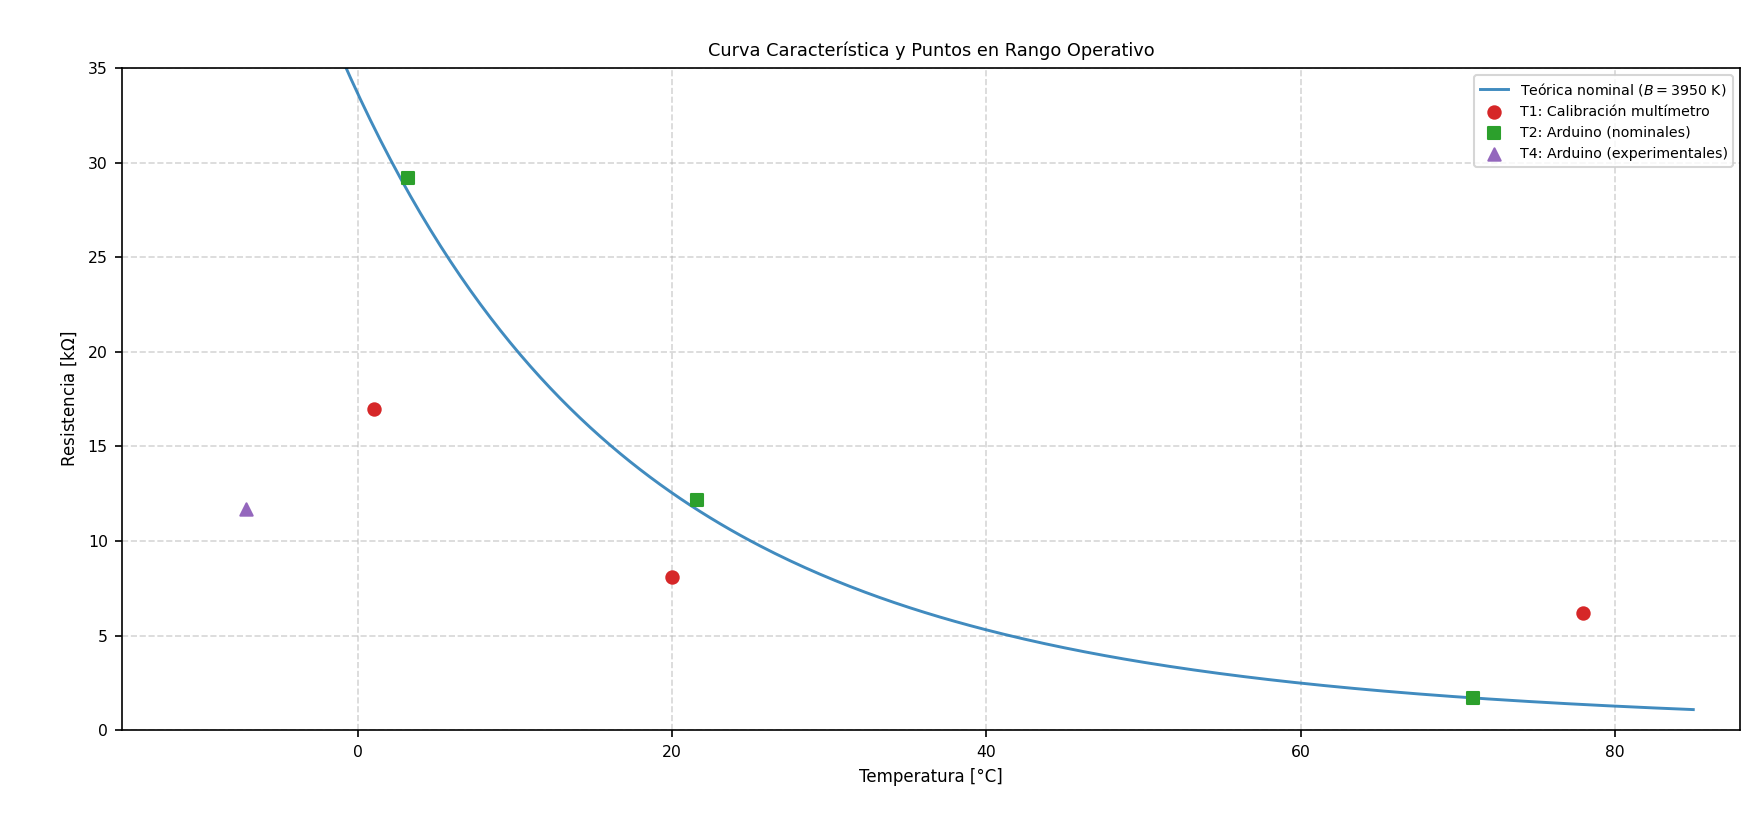
\includegraphics[width=0.95\textwidth]{figura_1_curva.png}
    \caption{Curva característica teórica nominal ($B = 3950\text{ K}$) y distribución de los puntos relevados en el rango físico operativo.}
    \label{fig:curva_operativa}
\end{figure}

\subsection{Resultados de la medición con parámetros experimentales}

\begin{table}[H]
    \centering
    \caption{Mediciones obtenidas mediante Arduino utilizando las mediciones obtenidas experimentalmente.}
    \begin{tabular}{|l|c|c|}
        \hline
         & \textbf{Temperatura} & \textbf{Resistencia} \\ \hline
        Ambiente & \SI{-7.1}{\celsius} & \SI{11694}{\ohm} \\ \hline
        Frio & \SI{146.6}{\celsius} & \SI{30610}{\ohm} \\ \hline
        Caliente & \SI{-901.4}{\celsius} & \SI{2171}{\ohm} \\ \hline
    \end{tabular}
    \label{tab:mediciones_arduino_experimental}
\end{table}

\begin{figure}[H]
    \centering
    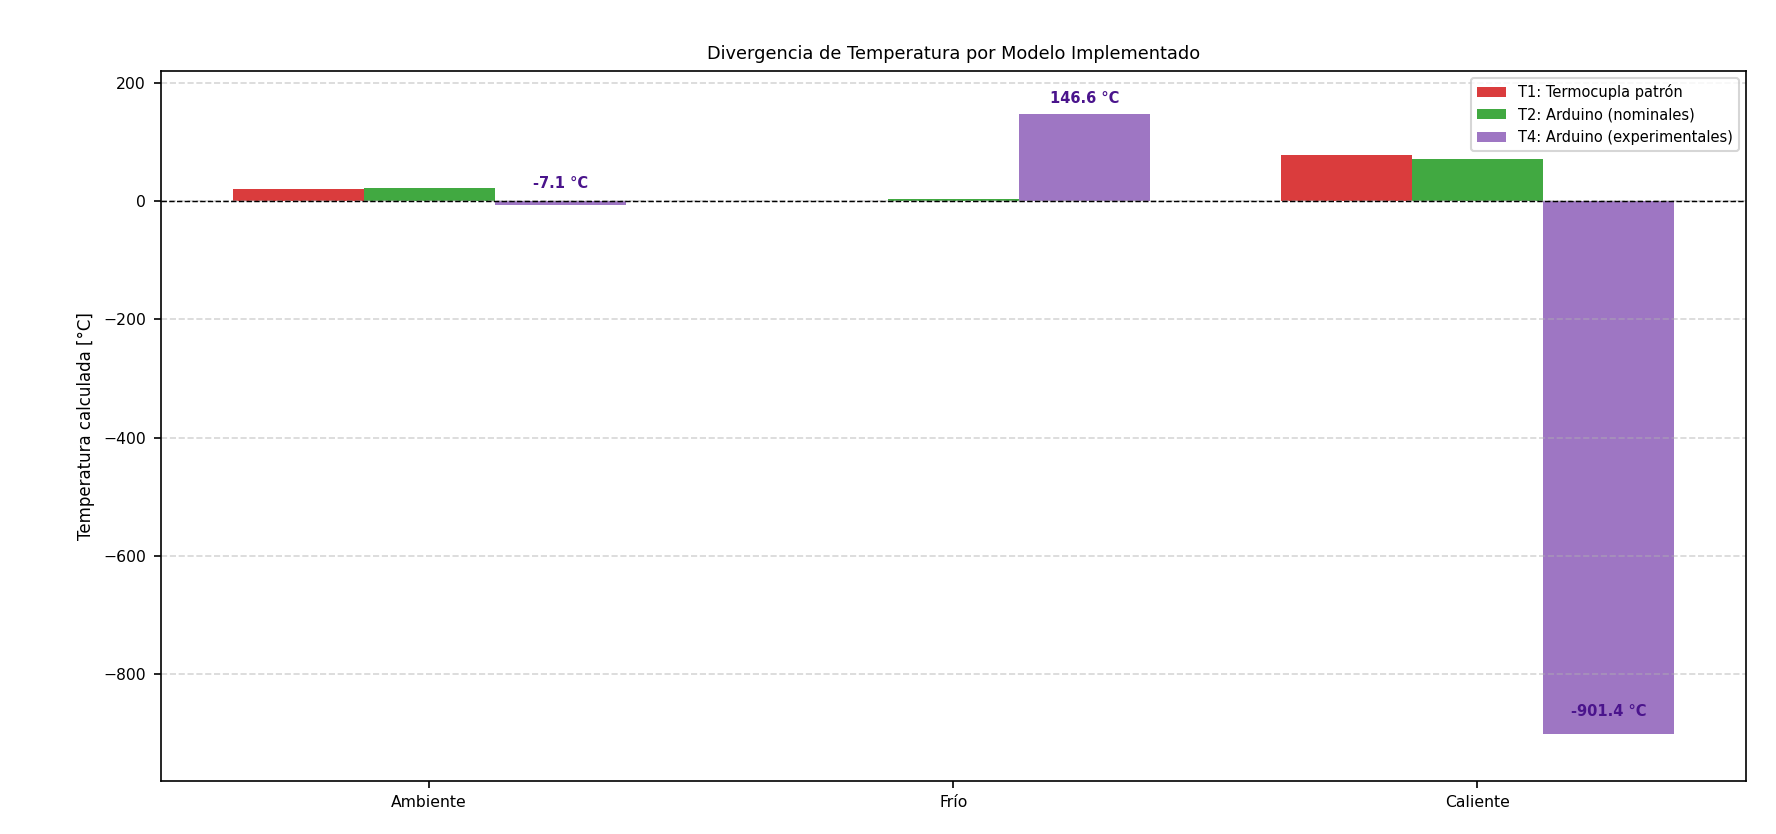
\includegraphics[width=0.95\textwidth]{figura_2_curva.png}
    \caption{Comparación de temperaturas obtenidas frente al patrón, evidenciando la divergencia originada por los coeficientes empíricos calculados.}
    \label{fig:divergencia_temperaturas}
\end{figure}


\end{document}
